\documentclass[a4paper,12pt]{article}
\usepackage[osf]{mathpazo}
\usepackage{ms}
\usepackage{amsmath,amsfonts,amssymb}
\usepackage{natbib}
\usepackage{lineno}
\usepackage{graphicx}
\usepackage{caption}
\modulolinenumbers[5]
\linenumbers

\pdfminorversion=3

\makeatletter
\renewcommand{\@biblabel}[1]{\quad#1.}
\makeatother

\title{Statistical and conceptual challenges in the comparative analysis of principal components}
\author{
Josef C. Uyeda$^{1,*}$, Daniel S. Caetano$^1$, and Matthew W. Pennell$^1$
}

\date{}
\affiliation{
 $^{1}$ Department of Biological Sciences \& Institute for Bioinformatics and Evolutionary Studies, University of Idaho, Moscow, ID 83844, U.S.A.\\ 
 $^{*}$ Email for correspondence: \texttt{pseudacris@gmail.com}\\
}

\runninghead{PCA in comparative analyses}
\keywords{Phylogenetic comparative methods, principal components, Brownian motion, Ornstein-Uhlenbeck, multivariate statistics}


\begin{document}

\mstitlepage
\parindent=1.5em
\addtolength{\parskip}{.3em}
\vfill

\section{Abstract}
\begin{enumerate}
\item A common procedure when analyzing multivariate data in a phylogenetic framework is to first transform the data into a set of principal component (PC) axes. Techniques for ``correcting for phylogeny'' when computing PCs have been developed and applied widely in the empirical literature. However, standard (i.e., uncorrected) principal components continue to be widely used in comparative analyses.

\item We demonstrate that failing to include phylogenetic relationships when calculating PC scores will mislead inferences in a predictable manner. Specifically, even when data are simulated under Brownian motion (BM), the first several PC scores will appear to have evolved rapidly early in a clade's history and slowed down towards the present day.

\item The primary method for calculating ``phylogenetically corrected'' PC scores relies on the assumption that the traits have evolved under a multivariate BM model. It is unknown whether this assumption is reasonable if the actual traits have evolved under more complex scenarios. Using simulations, we find that for many common models of evolution, calculating PC scores based on a BM model is a reasonable approximation though this approximation gets worse as the dimensionality of the analysis increases.

\item \emph{Synthesis:} While incorporating phylogeny when calculating PC scores does remove bias in many cases, a more fundamental issue remains when analyzing PCs in a comparative framework --- that drawing meaningful evolutionary inferences from models fit to PCs is challenging. Alternatives approaches for modeling multivariate data on a phylogeny are likely to be more informative, though further statistical and conceptual innovations will be necessary for these to be more broadly applicable.
\end{enumerate} 

\newpage

\section{Introduction}
The units of measurements are not neutral or arbitrary; different ways of representing the same set of data can change the meaning of the measurements and alter the interpretations of subsequent statistical analyses \citep{Hand2004, HansenHoule2008, Houle2011}. Therefore, careful attention needs to be paid to how data is measured and how it is transformed. Furthermore, this should be done with the scientific question in mind in order to ensure that resulting inferences are meaningful \citep{Houle2011}. 

Most approaches for studying evolution in a phylogenetic comparative framework were developed for univariate data \citep[reviewed in][]{PennellHarmon}. Even classical approaches for testing for correlated evolution across a phylogeny \citep[e.g.,][]{Felsenstein1985, Grafen1989, HarveyPagel1991} fundamentally model each trait as having evolved under an evolutionary process that is independent of the state of the other \citep{HansenOrzack2005}. However, the traits that we are actually interested in studying have likely evolved in concert with a suite of other traits and considering each trait is isolation may give a distorted picture of reality. Therefore, it is often desirable to reduce the multivariate dataset into a set of linear combinations of traits that are orthogonal to one another, such that each linear combination can then be analyzed with common comparative methods.

The most common method for reducing the dimensionality of the dataset is to perform Principal Components Analyses (PCA) prior to analyzing the data using phylogenetic comparative methods. The first PC axis is the eigenvector in the direction of greatest variance, the second PC axis, the second greatest variance, and so on. However, standard methods for calculating PC scores assume that the samples are independent of one another, which is hardly ever the case for comparative data --- as a result of shared common ancestry, relatives are likely to share many traits and trait combinations. This fact is of course, now almost universally recognized by biologists and conducting comparative analyses without considering the phylogenetic relationships of species is anathema to most evolutionary biologists. 

However, the necessity of considering phylogeny in some types of data transformations \citep{Revell2008} is not similarly recognized. Many researchers --- most of whom would never consider analyzing comparative data in a non--phylogenetic context --- continue the practice of conducting comparative analyses on standard PCs and thus inadvertently introduce substantial bias into their analyses. Typical examples of traits where this is done include geometric morphometric landmarks \citep[e.g.,][]{Dornburg2011, Hunt2013}, measurements of multiple morphological traits \citep[e.g.,][]{Harmon2010, BergmannIrshick2012, Weir2012, Pienaar2013, Price2014}, and climatic variables \citep[e.g.,][]{KozakWiens2010, Schnitzler2012}. We stress that the papers that we have cited here are simply examples (picked more--or--less, at random) from a substantial number of papers where this non--intuitive mistake was made.

Fortunately, multiple potential solutions exists to address this problem.  One frequently used method is that of \citet{Revell2008}, who developed a procedure (explained in detail below) for converting multivariate data into ``phylogenetically corrected'' PC axes (hereafter, pPCA), by assuming that the original data evolved along the phylogeny under a multivariate Brownian motion (BM) model of evolution. In a brief simulation study, \citet{Revell2008} demonstrated that if the underlying model for the traits was indeed a multivariate BM model, performing standard PCA gave biased estimates of the eigenvalues, whereas pPCA removed this bias.

In this brief contribution we first, extend the argument of \citet{Revell2008} and demonstrate that not only are the eigenvalues obtained from PCA biased but that they are biased in a systematic and predictable way. Performing comparative analyses on standard PC axes positively misleads inference. This point has been made in other fields that deal with autocorrelation between observations, such as population genetics \citep{Novembre}, ecology \citep{Podani2002}, climatology \citep{Richman1986} and paleobiology \citep{Bookstein2012}. However, the connection between these previous results and phylogenetic comparative data has not been explicitly made and standard PCs continue to be widely used in the field. We hope that our paper helps change this practice.

Second, as stated above, \citet{Revell2008} assumed that the measured traits had evolved under a multivariate BM model. This has the potential to introduce an odd circularity into the analysis. If we assume that the underlying traits have evolved under BM and calculate a set of pPC axes based on this assumption, it seems reasonable to suppose that if the true model of trait evolution were different, systematic biases in deviations from the BM model could generate predictable distortions across pPC scores that could affect inference of models of trait evolution. To our knowledge, the effect of this bias has not been explored. We perform a small simulation study to investigate this effect.

Last, we consider the interpretation of evolutionary models fit to pPC axes and discuss the conceptual and statistical advantages and disadvantages of using pPCA compared to alternative approaches for studying multivariate evolution in a phylogenetic comparative framework.

\section{Methods}
\subsection{\emph{Overview of pPCA}}
Before describing our analyses, we briefly overview the approach of \citet{Revell2008} for computing pPC scores for each species. In conventional PCA, a $m \times m$ covariance matrix $\mathbf{R}$ is computed from a matrix of trait values $\mathbf{X}$ for the $n$ species and $m$ traits
\begin{equation}\label{eq:rpca}
\mathbf{R} = (n-1)^{-1}(\mathbf{X} - \text{mean}[\mathbf{X}])^\intercal (\mathbf{X} - \text{mean}[\mathbf{X}]).
\end{equation}
We note that in many applications $\mathbf{X}$ may not represent the raw trait values; in geometric morphometrics, for example, size, translation and rotation will often be removed from $\mathbf{X}$ prior to computing $\mathbf{R}$ \citep{RohlfSlice, Bookstein1997}. The eigenvalues $\mathbf{D}$ and eigenvectors $\mathbf{V}$ of $\mathbf{R}$ are then obtained using singular--value decomposition $\mathbf{R}=\mathbf{V}\mathbf{D}\mathbf{V}^{-1}$ or some related technique. The scores $\mathbf{S}$, the trait values of the species along the PC axes are computed as
\begin{equation}\label{eq:Spca}
\mathbf{S}=(\mathbf{X} - \text{mean}[\mathbf{X}])\mathbf{V}.
\end{equation}

Phylogenetic PCA differs from this procedure in two important ways \citep{Revell2008,Polly2013} . First the covariance matrix is inversely weighted by the expected covariance of trait values between under a given model $\mathbf{\Sigma}$. Under a BM model of trait evolution, this is simply proportional to the structure of the phylogenetic tree, such that $\Sigma_{i,j}$ is the shared path length between lineages $i$ and $j$. Including the expected covariance between trait values essentially just re--orients the axes according to the phylogeny. Second, the space is centered on the ``phylogenetic means'' $\mathbf{a}$ of the traits rather than the arithmetic means. In pPCA, Equation \ref{eq:rpca} is therefore modified as
\begin{equation}\label{eq:rppca}
\mathbf{R} = (n-1)^{-1}(\mathbf{X} - \mathbf{1a}^\intercal)^\intercal \mathbf{\Sigma}^{-1} (\mathbf{X} - \mathbf{1a}^\intercal)
\end{equation}
where $\mathbf{a}=[(\mathbf{1}^\intercal \mathbf{\Sigma}^{-1} \mathbf{1})^{-1} 
\mathbf{1}^\intercal \mathbf{\Sigma}^{-1} \mathbf{X}]^\intercal$ \citep{RevellHarmon2008,Revell2008}. Similarly, $\mathbf{S}$ can be calculated for pPCA using Equation \ref{eq:Spca} but substituting the phylogenetic means for the arithmetic means
\begin{equation}\label{eq:Sppca}
\mathbf{S}=(\mathbf{X} - \mathbf{1a}^\intercal)\mathbf{V}
\end{equation}
where again, $\mathbf{V}$ is the eigenvectors of $\mathbf{R}$.

Two things are worth noting about the properties of pPCA. First while like PCA, the pPC axes are all orthogonal to each other, unlike PCA, the scores of each PC axis are not orthogonal to scores on other axes. Second, while the eigenvectors and eigenvalues of pPCA are indeed phylogenetically independent (assuming the model used to construct $\mathbf{\Sigma}$ is appropriate), the scores themselves are not \citep{Revell2008, Polly2013}. Both these properties imply that when testing for correlated evolution between pPC scores or between pPC scores from one axis an another trait, it is necessary to perform a phylogenetic analyses, just as one would with another other trait.  


\subsection{\emph{Simulations}}
\subsubsection{Effect of PCA on model selection under multivariate Brownian motion}
We simulated 100 replicate datasets under multivariate Brownian motion to evaluate the effect of standard and phylogenetic PCA on inference of the tempo and mode of phenotypic evolution. For each dataset, we simulated a pure-birth phylogeny of 50 terminal taxa scaled to unit height. We then simulated a 20-trait dataset under multi-variate Brownian motion. To generate the stepwise covariance matrix of the multivariate BM process $\mathbf{\Sigma}$, we simulated positive definite covariance matrices by drawing eigenvalues from an exponential distribution with a rate parameter of $\lambda = 1/100$ and simulating randomly oriented orthogonal eigenvectors. Data were then generated by drawing tip data a multivariate normal distribution with a variance-covariance matrix generated from the Kronecker product of $\mathbf{C}$ and $\mathbf{\Sigma}$.

For each of the 100 replicate datasets we fit either an BM, Early-Burst (EB) or Ornstein-Uhlenbeck with a fixed root (OU) model using the package \textit{phylolm} \citep{HoandAne2014}. These models were fit to each of the three transformations of each replicate dataset: the untransformed trait data, scores obtained from standard PCA and scores obtained from phylogenetic PCA. We then calculated the Akaike weights of each of the three models (BM, OU and EB) for each data transformation. 

\subsubsection{Effect of PCA when the generating model is not BM}
We conducted an additional set of simulations in which we varied the underlying model for each of the traits in the dataset. Because of difficulties in efficiently simulating large multivariate datasets of covarying traits under OU or EB models, we instead simulated 20 independent traits under either BM, OU or EB for 50 taxa trees (simulated as above). In each simulation, traits were simulated under only one model of evolution, with common parameters (BM: $\sigma^2 = 1$; EB: $a = log(0.02), \sigma^2 = 1$; OU: $\alpha=2, \sigma^2 = 1$). We then again fit either BM, EB or OU models using \textit{phylolm} and estimated parameters and Akaike weights for models fit to the original data, PCA scores, or pPCA scores. In addition to model-fitting, we conducted a node-height tests to determine whether phylogenetically independent contrasts were correlated to the height of the node for each of the 20 traits for either the original dataset, the PCs, or the pPCs. In addition, we generated disparity through time plots for each transformation of the data across each of the 20 traits. 

\subsection{\emph{Empirical examples}}


\section{Results}
\subsection{\emph{Simulations}}
\subsubsection{Effect of PCA on model selection under multivariate Brownian motion}
PCA introduces a systematic bias in the favored model across principal components. In our simulations, EB models had systematically elevated support as measured by Akaike weights for the first few components, for which it generally exceeded support for the BM model \ref{corbm}. Fitting models sequentially across PC axes 1-20 revealed a regular pattern of increasing support for first BM models toward intermediate components, followed by increasing support for OU models among later components (which generally approached 1). This regular pattern across trait axes was not present for either the original datasets, or for phylogenetic principal components, which found strong support for the BM model regardless of which trait was analyzed (note that the theoretical maximum for Akaike weights for the BM model is $\sim 0.576$, as BM is a special case of the OU and EB models when $\alpha=0$ or $a = 0$, respectively, and cannot have a higher likelihood than either of these models).   

\subsubsection{Effect of PCA when the generating model is not BM}
If the underlying model was either OU or EB rather than BM, then phylogenetic PCA tended to increase support for the true model relative to the original trait variables for the first few component axes (Supplementary Figures \ref{aicwbm}, \ref{aicweb}, \ref{aicwou}). For example, when each of the original trait variables were simulated under an OU process, support for the OU model increased for pPC1 relative to the original trait variables. Higher principal component axes inferred a regular pattern of decreasing support for the OU model, with the last few PCs have equivocal support for either a BM or OU model \ref{oufit}. Furthermore, estimation of parameters was affected by phylogenetic PCA, with higher values of $\alpha$ estimated for the first few pPC scores relative to the generating value of $\alpha=2$ for the original traits. This estimate of $\alpha$ decreased for higher components until the estimated value appeared essentially equivalent BM trait evolution. 

The effects of PCA and phylogenetic PCA become more apparent by conducting a node height test, which compares the values of phylogenetically independent contrasts against the height of the nodes at which they are measured (Figure \ref{nhplot}, \citealt{Freckleton2006}). Under OU models, traits are expected to have the highest contrasts near the tips, while under EB models, traits will have the highest contrasts near the root of the tree. Standard PCA tends to select linear combinations of traits that maximize the contrasts at the root of the tree, thereby maximizing the overall variance explained across the entire dataset. Thus, the first few PCs are skewed toward resembling EB models, while the last few PCs are skewed toward resembling OU models. By contrast, the effect of pPCA on the node-height relationship depends on the generating model. When traits are evolved under an OU model, then the slope of the first PC vs. time is exaggerated to an even higher value. When traits are evolved under an EB model, the slope is likewise exaggerated, but toward higher magnitude negative values. This slope flattens out for increasing pPC axes. This pattern is further reflected in mean relative disparity through time, which measures the amount of variation present at time slices across the phylogeny relative to the total variance at the tips. Again, when standard PCA is used, or when the model is misspecified when calculating pPCA, then we observe predictable distortions of disparity through time across increasing pPC trait axes (Figure \ref{dttplot}). 

\subsection{\emph{Empirical examples}}

\section{Discussion}
\subsection{\emph{Standard PCA should not be used for comparative analyses}} 

The effect of computing PC scores on phylogenetically correlated data has not been widely appreciated, largely because PCA is viewed as a benign linear transformation of multivariate data. Certainly, when used as a descriptive tool, PCA can be broadly used even when assumptions regarding statistical non-independence or multivariate normality are violated \citep{Jolliffe2002}. Thus, there is nothing inherently wrong with using standard PCA or phylogenetic PCA on comparative data to describe axes of maximal variation across species or for visualizing divergence across phylomorphospace \citep{Sidlauskas2008}. However, we show that using PCA for inference from non-independent observations is considerably more problematic \citep{Jolliffe2002}. 

An intuitive understanding of the effect of PCA can be obtained by considering a multivariate BM process on a phylogeny. Despite a constant stochastic rate of evolution across each dimension of trait space, stochasticity will ensure that some dimensions will diverge more rapidly than expected early in the phylogeny, while others will diverge less. All else being equal, dimensions that happen to diverge early are expected to have the greatest variance across species, and standard PCA will identify these axes as the primary axes of variation. However, once these trait axes are selected, ``regression toward the mean'' ensures that the chance elevation of rates that occurred early on in the phylogeny is unlikely to be maintained, resulting in a characteristic ``Early-Burst'' pattern of evolution for the first few principal components. An analogous process will result in the last few PCs following an OU process, in which the amount of divergence will appear to increase toward the present. Standard PCA thus ``sorts'' orthogonal trait dimensions by whether they follow EB, BM and finally, OU like patterns of trait divergence. Thus, meaningful conclusions regarding either slow-downs or accelerations of trait evolution cannot be made from univariate PC scores inferred from standard PCA. 

\subsection{\emph{Using pPCA when trait evolution is non-Brownian}}
In his original pPCA method, \citet{Revell2008} assumed that the original traits evolved under a multivariate BM model. Under this assumption, phylogenetic PCA mitigates the biased selection of PC axes by scaling divergence by the expected divergence given the branch lengths of the phylogeny. When the true model of evolution is not BM, then systematic deviations will be magnified by pPCA, and result in predictable distortions across pPC axes. We find that these distortions primarily serve to inflate the support for the true model of trait evolution when all dimensions follow a common model, which in and of itself is not suboptimal behavior (we expect stronger support for models with larger datasets). However, regular and predictable distortions across trait axes confound interpretation of the evolutionary model and estimated parameters (Figures \ref{nhplot} and \ref{dttplot}). 

\cite{Revell2008} suggested that alternative covariance structures could be used to estimate phylogenetically independent PCs for different models. For example, one could first optimize the $\lambda$ model \citep{Pagel1999} across all traits simultaneously \citep[using the method of][]{Freckleton2002} and then rescale the branch lengths of the tree according to the estimated parameter in order to obtain $\mathbf{\Sigma}$ for use in Equation \ref{eq:rppca}. However, model comparisons across alternative linear combinations of traits are not meaningful.  Furthermore, as noted by \citet{Revell2008}, parameters estimated to construct the covariance structure for the pPCA will likely be different from the same parameters estimated using the PC scores themselves. Additionally, while this method is restricted to models that assume a shared mean and variance structure across traits \citep[see][for examples where this does not  apply]{Hansen2008, Bartoszek2012}. 

Consequently, it is unclear how assuming relatively simple models such as BM to define pPC axes will affect inference using complex models of trait evolution, which are increasingly being applied in phylogenetic comparative analyses (cite). At a minimum, it seems likely that regular changes in evolutionary temp and mode should be expected when progressing from one pPC axis to the next, merely as a result of model misspecification and the biased selection of stochastic events into particular pPC axes.   

These results certainly do not imply that the biological inferences made from analyzing standard PC scores in a comparative framework are necessarily incorrect. %Effect may be small when low dimensional
Interestingly, when \citet{Harmon2010} analyzed the evolution of PC2 (what they referred to as ``shape'') obtained using standard PCA, they found very little support for the ``Early Burst'' model \citep{Blomberg2003} across their 39 datasets. The fact that their use of standard PC axes biased their results \emph{towards an ``Early Burst'' pattern} only serves to strengthen their overall conclusion that such slowdowns are indeed rare \citep[but see][]{SlaterPennell}. However, our results do suggest that in some cases, analyses conducted with PC axes should perhaps be revisited to ensure that results are robust.

%Note that we only simulated under a very restricted set of conditions.

%Discussion of main results (both simulated and empirical)

%Tie into results from other studies (e.g., novembre)


\subsection{\emph{The interpretation of pPCA}}

Aside from the statistical issues raised here, a broader, and more interesting, question is how one should draw evolutionary inferences from models of trait evolution fit to pPC axes. While principal components are convenient representations of multivariate data in univariate space, this comes at the cost of abstracting the data that is analyzed from the questions that are asked. 

First, using principal components often divorces model fitting from the study of interpretable evolutionary processes. If we treat the PC scores as a univariate trait than we are only considering divergence along the PC axis. This is sensible from a purely statistical standpoint but in doing so, we may miss a great deal about what is actually going on in the data. The first principal component axis computed from comparative data is the major axis of divergence across a clade (also known as the ``line of divergence''). This axis is of considerable interest in evolutionary biology. The direction of this line of divergence may be affected by the orientation of within--population additive genetic (co)variance $\mathbf{G}$, such that evolutionary trajectories may be biased along ``genetic lines of least resistance'' \citep[i.e., divergence occurs primarily along the leading eigenvector of $\mathbf{G}$, $G_{\text{max}}$;][]{Schluter1996, Arnoldetal2001}. Alternatively, the line of divergence may align with the ``selective lines of least resistance'', due to the structure of phenotypic adaptive landscapes \citep{Arnold2003, Jonesetal2007, Arnoldetal2008}, or else may be driven by patterns of gene flow between populations \citep{Guillaume2007} or the pleiotropic effects of new mutations \citep{Jonesetal2007, Hether2013, Houle2013}. Furthermore, pleiotropy and the genetic covariance between traits has been proposed as a potential resolution to the ``paradox of stasis'' \citep{HansenHoule2004}; traits with abundant within--population additive genetic variation may be constrained over macroevolutionary time scales \citep{Kirkpatrick2009, WalshBlows2009}. Phylogenetic comparative data can potentially provide unique and novel insights into the connection between micro-- and macroevolution \citep{Hohenlohe2008} but such questions can only be addressed in a truly multivariate context. While the traits identified by PCA will be statistically orthogonal (assuming that the model of evolution used for the transformation is appropriate; see above), this only true in the particular snapshot captured by comparative data and should not be taken to imply that they are evolving independently. 

%% Replaced this paragraph
%The first principal component axis of comparative data can be considered the major axis of diversification of a clade (often called the ``line of divergence"). This axis is of considerable interest to evolutionary biology, as it may be affected by the structure of within-population genetic variation, or the G-matrix ($\mathbf{G}$) \citep{Schluter1996}. The leading eigenvector of the additive genetic variance-covariance matrix ($G_{max}$) may bias evolution along ``genetic lines of least resistance" \citep{Schluter1996, Arnoldetal2001}. Alternatively, it is possible that alignment (or mis-alignment) between the eigenvectors of $\mathbf{G}$ and the line of divergence can result from ``selective lines of least resistance", which describe the path of least resistance along phenotypic adaptive landscapes \citep{Arnold2003, Jonesetal2007, Arnoldetal2008}. Potentially complicating the issue even further, continued gene flow and migration can result in alignment of divergent populations \citep{Guillaume2007} as can the structure of the mutational variance-covariance matrix \citep{Jonesetal2007, Hether2013}. For these reasons, testing for alignment or mis-alignment of $G_{max}$ and the line of divergence is of significant interest toward connecting micro- and macroevolution \citep{Hohenlohe2008}. However, such questions are not easily removed from a truly multivariate framework and our intuitions based on two and three trait cases do not scale well to higher dimensions. We have shown that reducing highly multivariate stochastic evolutionary models to a few principal components runs the risk of conflating evolutionary noise with evolutionary process; making interpretation of parameters and model-fits difficult at best, and abstracting the traits under study from the models being tested. 

For some macroevolutionary questions, evolutionary processes may not be of primary interest and the loss of information when using PCs may be acceptable. For instance, if the goal of fitting and comparing models is to make broad inferences about evolutionary patterns, such as the ``rate'' of trait evolution \citep{Freckleton2011, Hunt2012}, then we may not care if the models are connected to any process. Many commonly used trait models \citep[notably, the ``Pagel'' tree transformations $\lambda, \delta, \kappa$;][]{Pagel1997, Pagel1999} have no real bearing on any evolutionary processes anyways \citep{HansenOrzack2005} and therefore using PCs in conjunction with these models therefore does not seem to come at a great cost. Other models, can be tied to specific evolutionary processes \citep{HansenMartins1996, EstesArnold2007, Hansen2008, Hansen2012SysBio, PennellHarmon, PennellPE} and using PC axes necessarily breaks this tie.

Second, phenotypes are the ``stuff'' of evolution, not PC axes. Researchers often use broad terms to translate the PC axes back to trait space, such as stating that PC1 represents size and PC2, shape \citep[e.g.,][]{Harmon2010, Price2014}. However, this is a very imprecise way of quantifying biologically interesting variation. It is often difficult to understand exactly what we are explaining when we find that the evolution of PC2 is well described by, say, an OU process.

\subsection{\emph{What are the alternatives?}}

A number of alternative approaches may be used to study the evolution of correlated phenotypes along a phylogeny. The most conceptually straightforward alternative is to construct models in which there is a covariance in trait values between species (which is done in univariate models) and a covariance between different traits. Such multivariate extensions of common quantitative trait models have been developed \citep{RevellHarmon2008, Hohenlohe2008, RevellCollar2009, ButlerKing2009, motmot}. These allow researchers to investigate the connections between lines of divergence and within--population evolutionary parameters \citep{Hohenlohe2008} as well as to study how the correlation structure between traits itself changes across the phylogeny \citep{RevellCollar2009}. 

However, these approaches also have substantial drawbacks. First, the number of free parameters of the models rapidly increases as more traits are added \citep{RevellHarmon2008}, making them impractical for large multivariate datasets. Second, these models allow for inference of the covariance between traits but the cause of this covariance is usually not tied to specific evolutionary processes. The first issue may be addressed by constraining the model in meaningful ways \citep{ButlerKing2009} or by assuming that \emph{all traits} have the same covariance structure \citep{Adams2014, Adams2014b}; similarly, one could divide the traits into sets a priori and then assume that all traits in a set have a common variance structure \citep{Klingenberg2013}. Such restrictions of parameter space are especially appropriate for truly high--dimensional traits, such as shape inferred from geometric morphometric landmark data, for which we are primarily interested in the evolution of the aggregate trait and not necessarily the individual components. The second (inferential) difficulty can be addressed by explicitly modeling the evolution of some traits as a response to evolution or others. Hansen and colleagues have developed a number of models in which a predictor variable evolves via some process and a response variable tracks the evolution of the first as OU process \citep{Hansen2008, Labra2009, Hansen2012SysBio, Bartoszek2012}. This has been a particularly useful way of modeling the evolution of allometries \citep{Hansen2012SysBio, Voje2013, Voje2013b}. However, like the ``covariance''  models discussed above, increasing the number of traits makes the model much more complex and difficult to fit.

%For analyses of multivariate trait data, it is fairly straightforward to construct multivariate forms of commonly used trait models (e.g., BM, OU, etc.). In the univariate case, one must estimate a vcv matrix ($\mathbf{\Sigma}$ above) representing the expected variances and covariances between taxa for the trait being studied \citep[see][for details]{Harmon2010, Omeara2012}. In the multivariate case, $\mathbf{\Sigma}$ is the expected variances and covariance between all taxa and all traits \citep{RevellHarmon2008, Hohenlohe2008, RevellCollar2009, ButlerKing2009, motmot}. For the simple case of multivariate BM, fitting this model requires computing the Kronecker product of $\mathbf{R}$ (from Equation \ref{eq:r}) and $\mathbf{C}$, the patristic distance matrix derived from the phylogeny (that is, $\mathbf{\Sigma} = \mathbf{R} \otimes \mathbf{C}$). $\mathbf{\Sigma}$ is therefore a $nm \times nm$ matrix (where as above, $n$ is the number of species in the phylogeny and $m$ is the number of measured traits). While parameters may be constrained ,such as forcing several traits to share the same variance structure in an OU model, clearly the number of parameters increases very quickly as more traits are included.

%A more biologically realistic alternative is to directly model the evolution of one trait as a response to the evolution of other traits (rather than just testing whether they are correlated). Hansen and colleagues have developed a number of models in which a predictor variable evolves via some process and a response variable tracks the evolution of the first as OU process \citep{Hansen2008, Labra2009, Hansen2012SysBio, Bartoszek2012}. This has been a particular useful way of modeling the evolution of allometries \citep{Hansen2012SysBio, Voje2013, Voje2013b}. However, like the correlational models discussed above, increasing the number of traits makes the model much more complex and difficult to fit.

For these reasons, it often remains necessary to reduce the dimensionality of a multivariate dataset to one or a few compound traits. We argue that PCA can be potentially quite usefully applied to this problem, though in ways that are statistically and conceptually distinct from how it is conventionally applied to comparative data. One potential approach is to use principal components computed from within--population data, rather than comparative data. For example, if $\mathbf{G}$ (or failing that, the phenotypic variance--covariance matrix $\mathbf{P}$) is available for a focal species, then the principal axes of variation in a focal species can be measured across all species in the phylogeny. Therefore, all measurements are defined relative to a particular species' primary axes of genetic variation. This removes biases in selection of PCs that result from phylogenetic structure and stochastic evolutionary models, and focuses the study on a trait with a known relationship to other traits (at least for a focal species). 

Another alternative is to use PCA as an exploratory tool to select interpretable linear combinations of traits of biological interest. Interpretation of principal components is often approximated by visually truncating the loadings to discrete values. In practice, such interpretation is sometimes quite obvious, and sometimes akin to reading tea leaves. More rigorous algorithms can be applied to identify subsets of the original variables that best approximate the principal components, which are frequently more interpretable \citep{Cadima2001}, while the second and third may correspond to identifiable contrasts between morphological measurements. However, the first PC will include not only overall size, but also some elements of shape and stochastic noise \citep{Somers1986, Somers1989}. If the primary axis appears well--correlated to a measure of overall body size, then a number of alternatives exist for explicitly measuring or removing size from the analysis that do not confound size with the limitations of PCA \citep{Somers1989}. Other alternatives to PCA for increasing interpretability include methods such as components with discrete-valued coefficients \citep{Hausman1982}, simple component analysis where coefficients are restricted to integers \citep{Vines2000}, or sparse principal components which shrink coefficients to zero below a specified tuning parameter \citep{Jolliffe2002, Zou2006}. It should be noted that increasing interpretability of linear combinations of traits does not eliminate the effects we have described in this manuscript. Components that are chosen using any of these methods without regard for the non-independence introduced by phylogeny will be likely biased in ways similar to traits identified with standard PCs. However, such procedures can at least increase the likelihood that the biased inferences made are intepretable and of biological interest (which reduces selection of components to a more general practice in biology--the selection of a biased sample of interesting traits).  

Of course, components defined by within--population variance structure or by approximating principal components with interpretable linear combinations will not explain as much variance across taxa as standard PCA and will not be orthogonal. However, the extra variance explained by the principal components of comparative data may in fact include a sizeable amount of stochastic noise, rather than interesting biological trait variation (as we have shown in our simulations). We argue that the added intepretability of carefully chosen and biologically meaningful trait combinations far outweighs the cost of slight collinearity or explaining less--than--maximal variation.

\section{Concluding remarks}
In this note, we sought to clarify some statistical and conceptually issues regarding the use of principal components in comparative biology. We have shown that from a statistical standpoint, failing to consider the phylogeny when performing PCA can be positively misleading. And despite the development of methods to correct for this, in our reading of the empirical literature, we have found this to be a common oversight. A secondary aim of our paper was to provoke a discussion about how we should go about analyzing comparative data. We certainly do not have the answers but believe there are some major theoretical limitations in using PCA (phylogenetic or not) to analyze comparative data. We think that we, as a field, need to think hard about what questions we can ask with multivariate comparative data and what types of measurements will allow us to address them.

\begin{figure}[p]
\centering
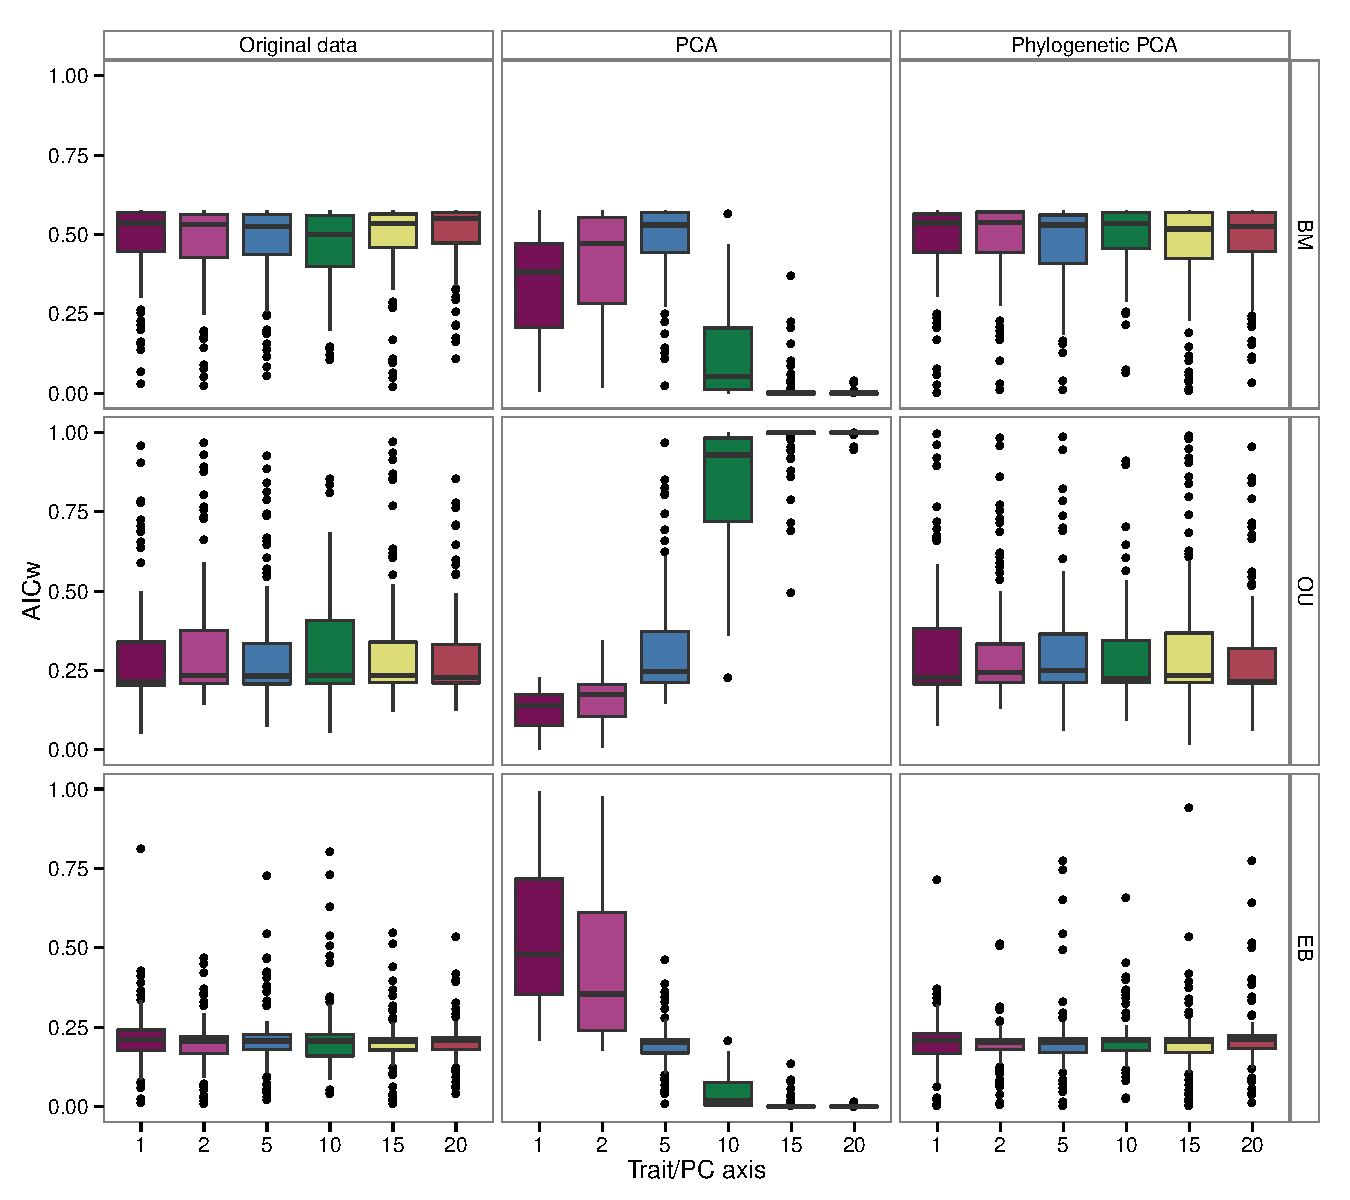
\includegraphics[scale=0.5]{./fig/box-aicw-corbm.pdf}
\caption{Distribution of Akaike weights for the Brownian motion (top row), Ornstein-Uhlenbeck (middle row) or Early-Burst model (bottom row). Models were fit to each replicated dataset for each of 6 different traits which were taken either from the original data (left column), PC scores (middle column) or phylogenetic PC scores (right column). Boxplots indicate the distribution of Akaike weights across each of 100 replicated datasets. Note that EB models have higher Akaike weights for the first few PCs of standard PCA, and that later PCs subsequently favor BM and finally, OU models. No such bias is found across traits for either the original data or pPCA.}
\label{corbm}
\end{figure}

\begin{figure}[p]
\centering
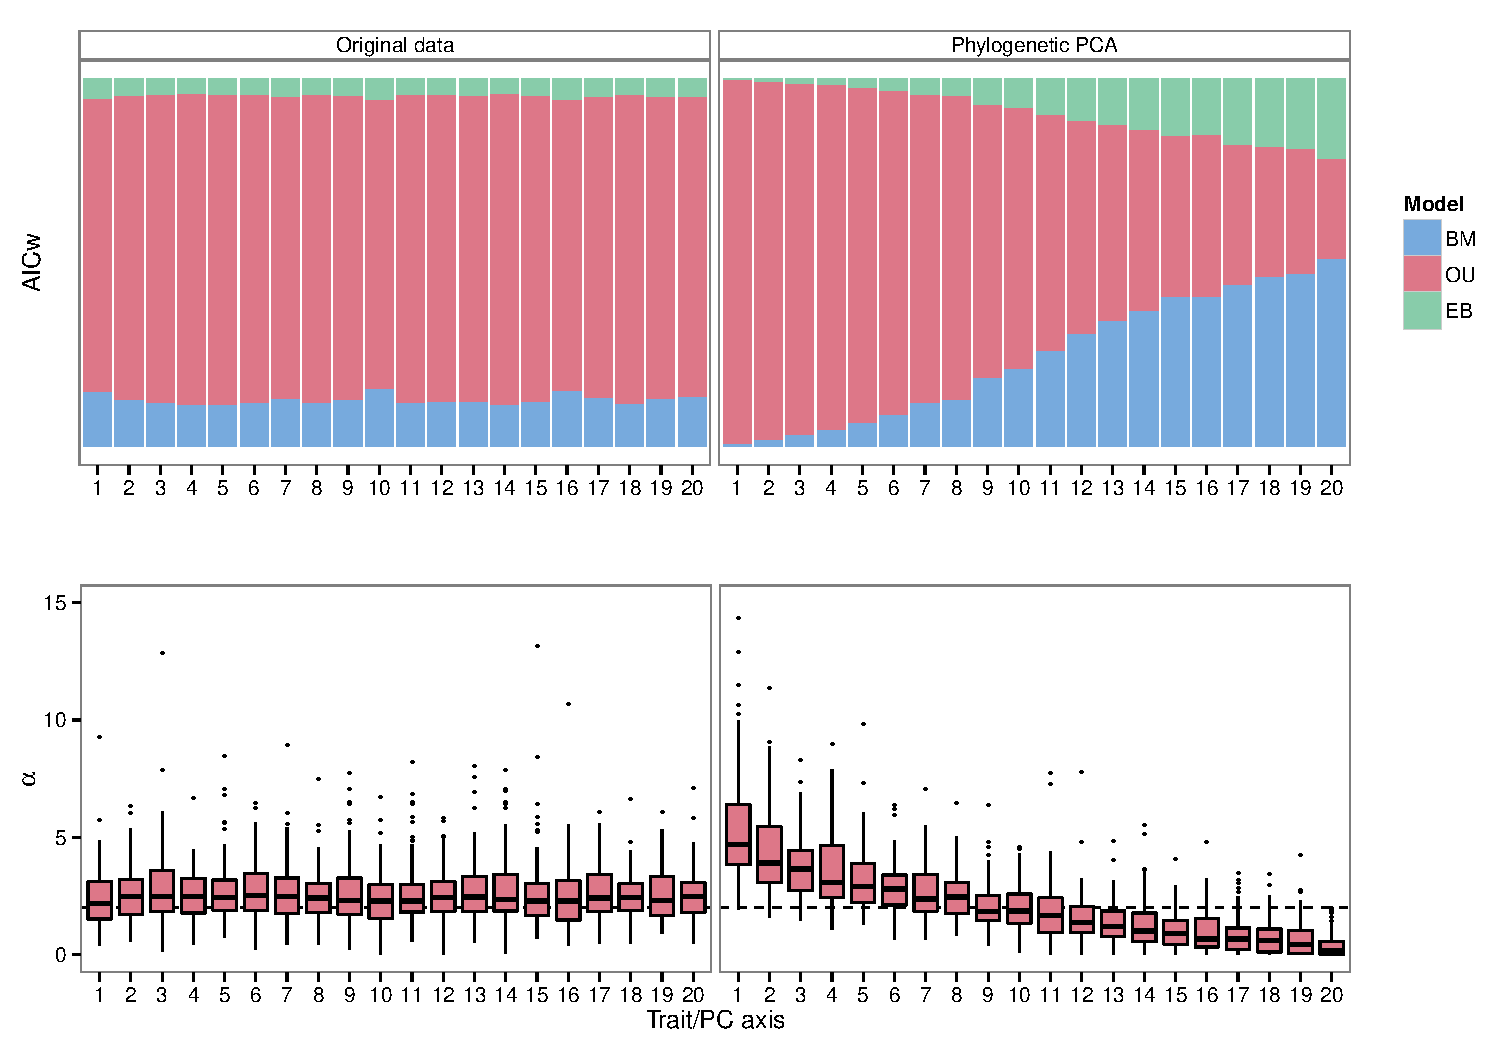
\includegraphics[scale=0.5]{./fig/model-support-alpha.pdf}
\caption{Akaike weights and parameter estimates for data simulated under an OU model, but subsequently fit using pPCA assuming multivariate BM. Akaike weights across traits (either original data, or pPCs) show a regular pattern of increasing support for BM and EB models for pPCA compared to the original traits (top row). Furthermore, while $\alpha$ and other parameters are well-estimated for the original traits, phylogenetic PCA produces a regular pattern of decreasing $\alpha$ values across pPC scores (bottom row). Note that the first few pPC axes have strong support for an OU model, and substantially higher estimates of $\alpha$ relative to the value used to generate the data (solid blue line, $\alpha = 2$). }
\label{oufit}
\end{figure}

\begin{figure}[p]
\centering
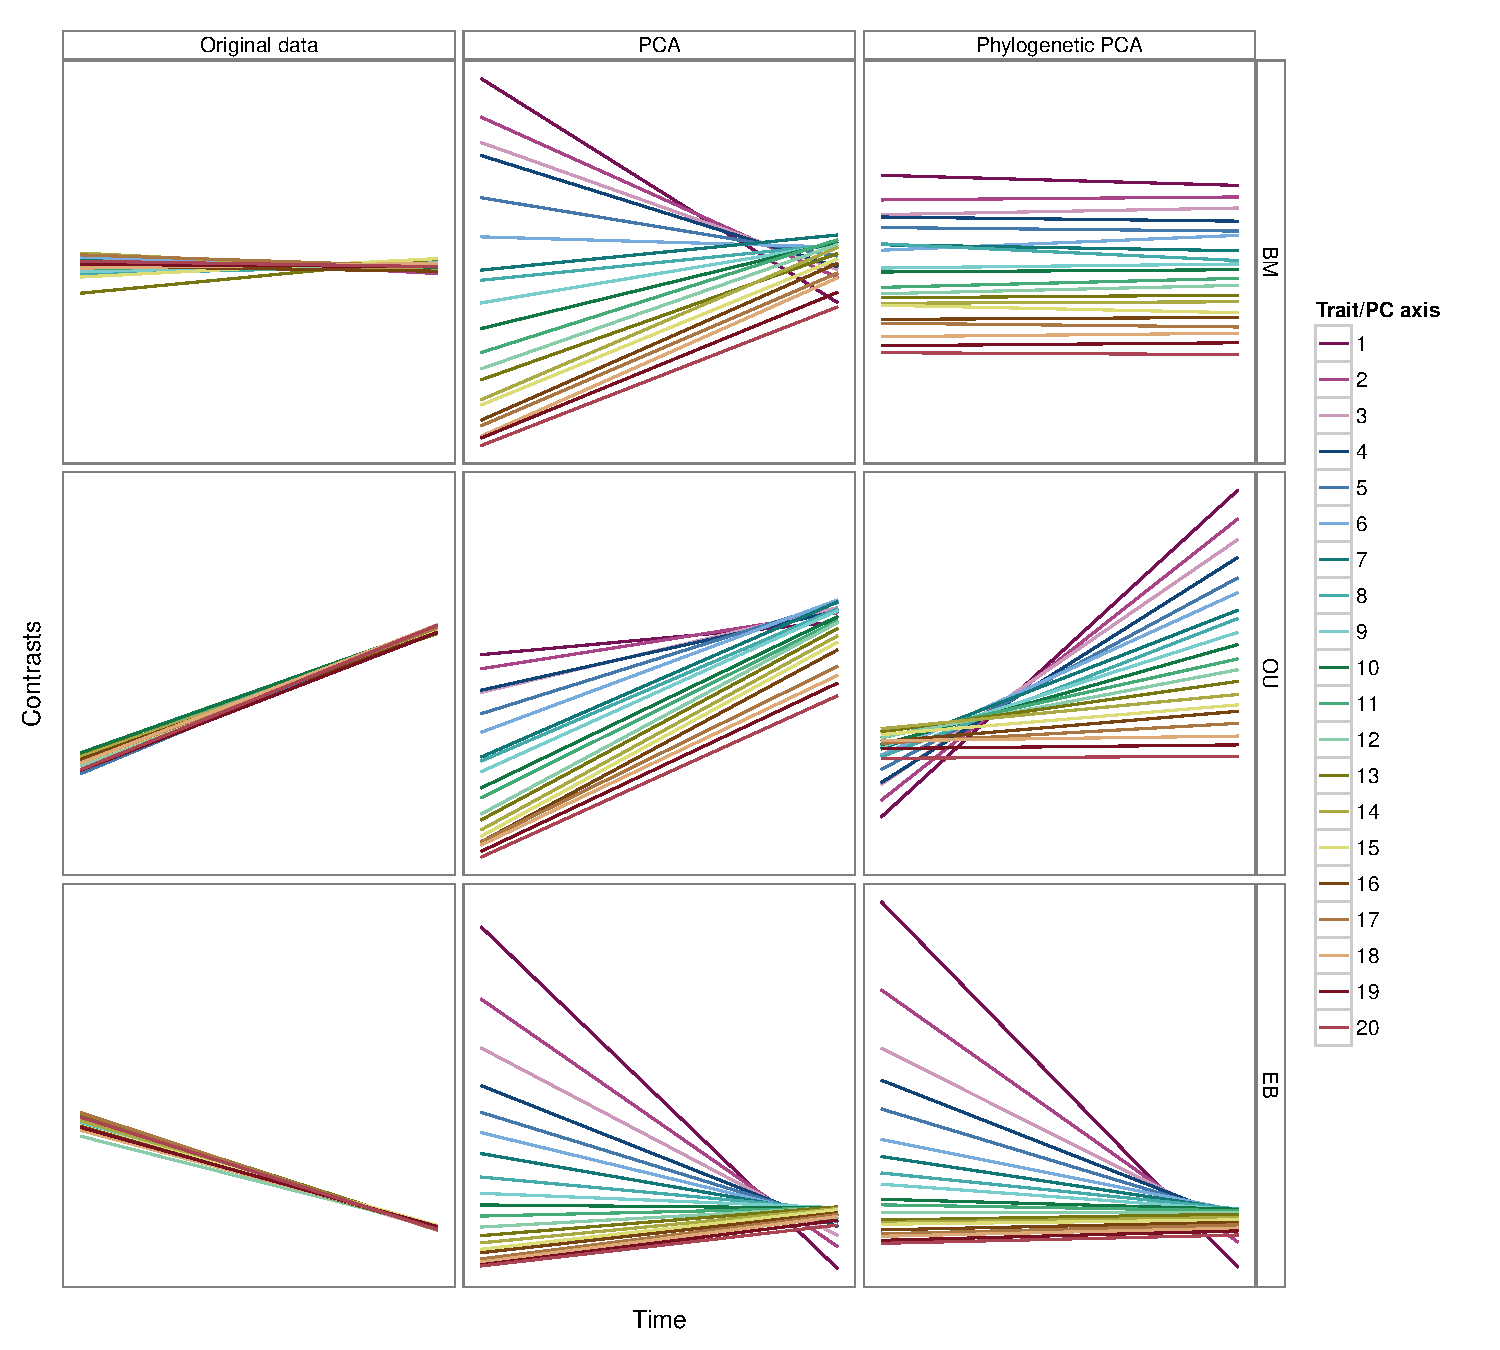
\includegraphics[scale=0.5]{./fig/nh-3models.pdf}
\caption{Relationship between the average phylogenetic independent contrasts and the height of the node across 100 datasets simulated under either a BM (top row), OU (middle row) or EB (bottom row) model of evolution. Contrasts were calculated for each of the 20 traits corresponding to either the original data (left column), PC scores (middle column) or pPPC scores (right column). Each line represents a best-fit linear model to the aggregated data across all 100 replicate simulations. The plots are oriented so that the left side of each panel corresponds to the root of the phylogeny, with time increasing tipward to the right. PCA results in a predictable pattern of increasing slope in the contrasts across PCs. By contrast, pPCA only has systematic distortions across pPC axes when the underlying model is not multivariate BM. When this occurs, the first few pPC axes tend to have more extreme slopes than the original data.}
\label{nhplot}
\end{figure}

\begin{figure}[p]
\centering
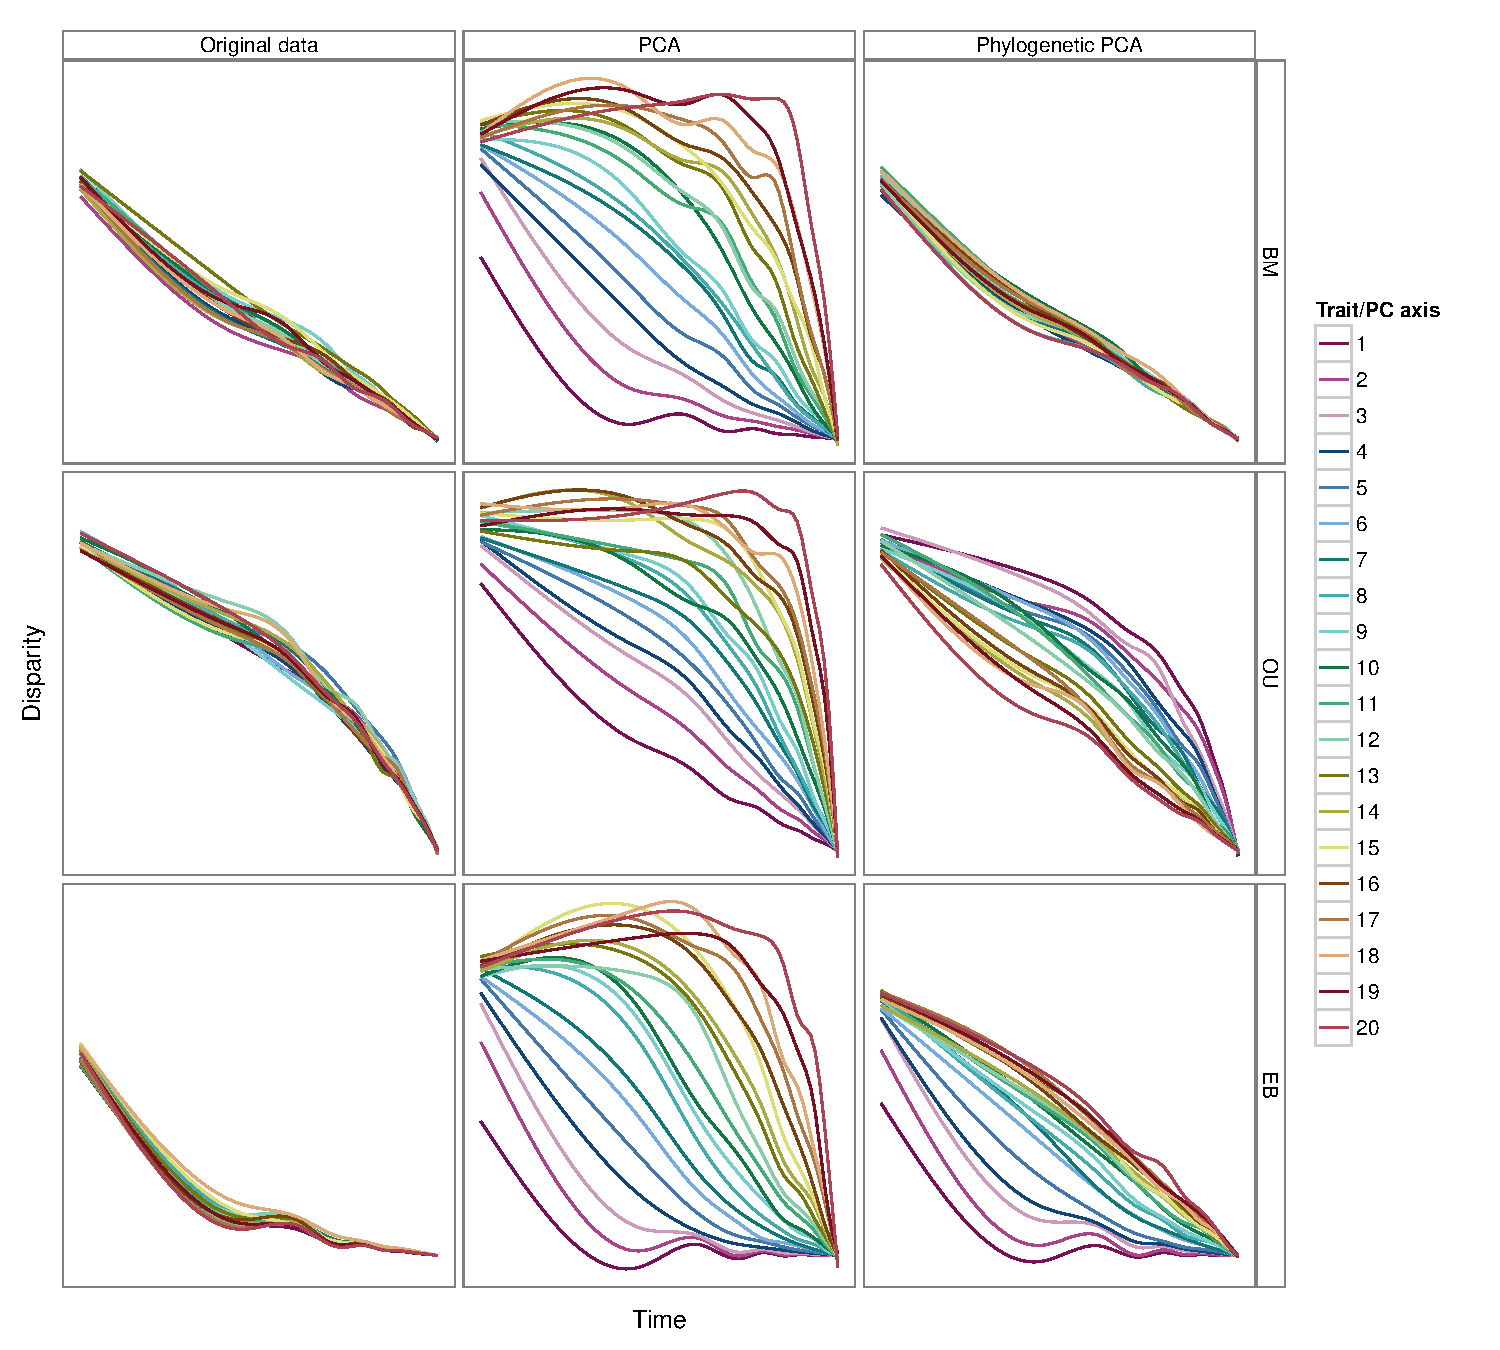
\includegraphics[scale=0.5]{./fig/dtt-3models.pdf}
\caption{Relative disparity through time for the same simulated datasets as in Figure \ref{nhplot}.}
\label{dttplot}
\end{figure}

\begin{figure}[p]
\centering
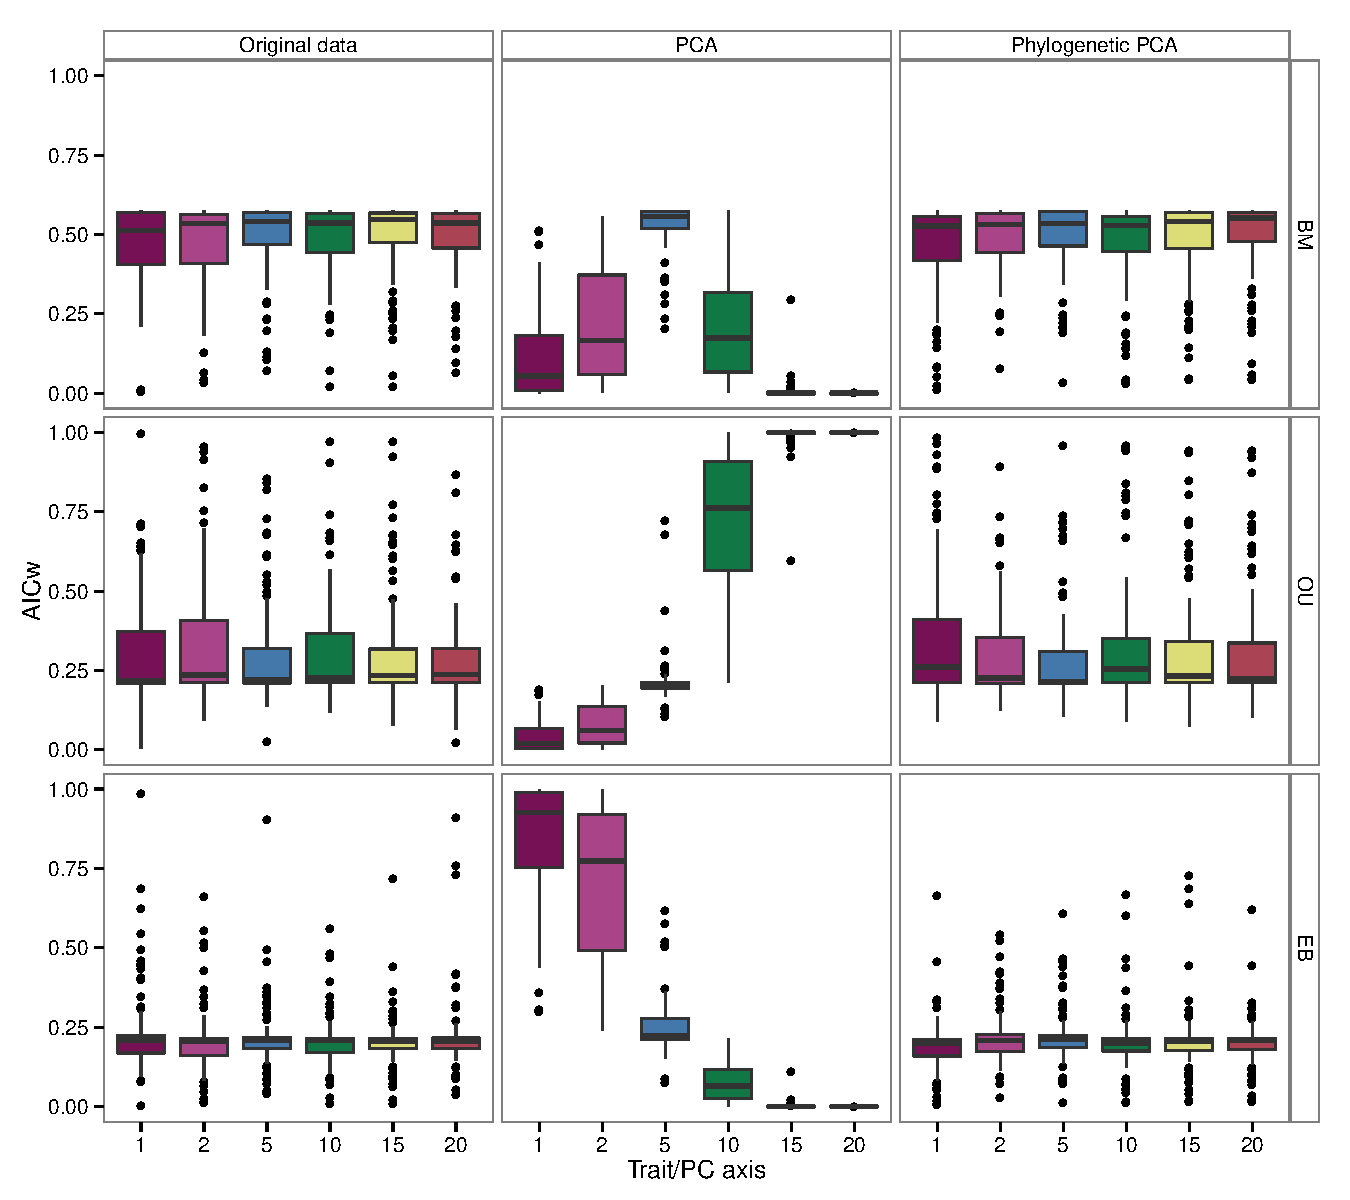
\includegraphics[scale=0.5]{./fig/box-aicw-mvbm.pdf}
\caption{}
\label{aicwbm}
\end{figure}

\begin{figure}[p]
\centering
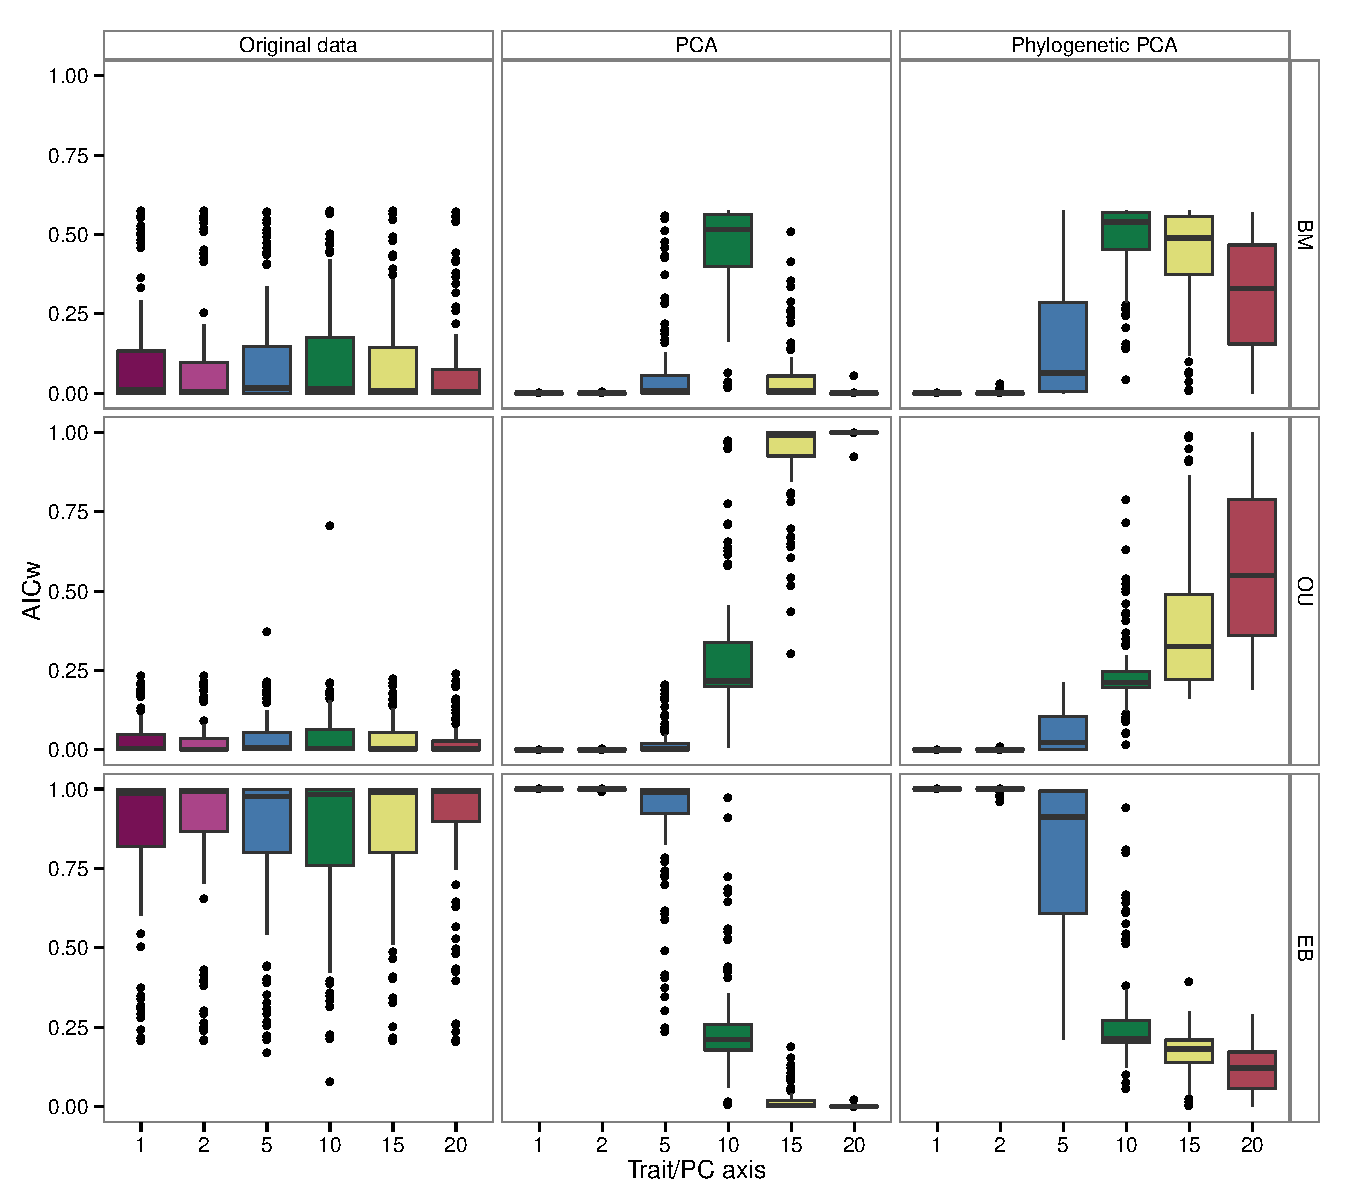
\includegraphics[scale=0.5]{./fig/box-aicw-mveb.pdf}
\caption{}
\label{aicweb}
\end{figure}

\begin{figure}[p]
\centering
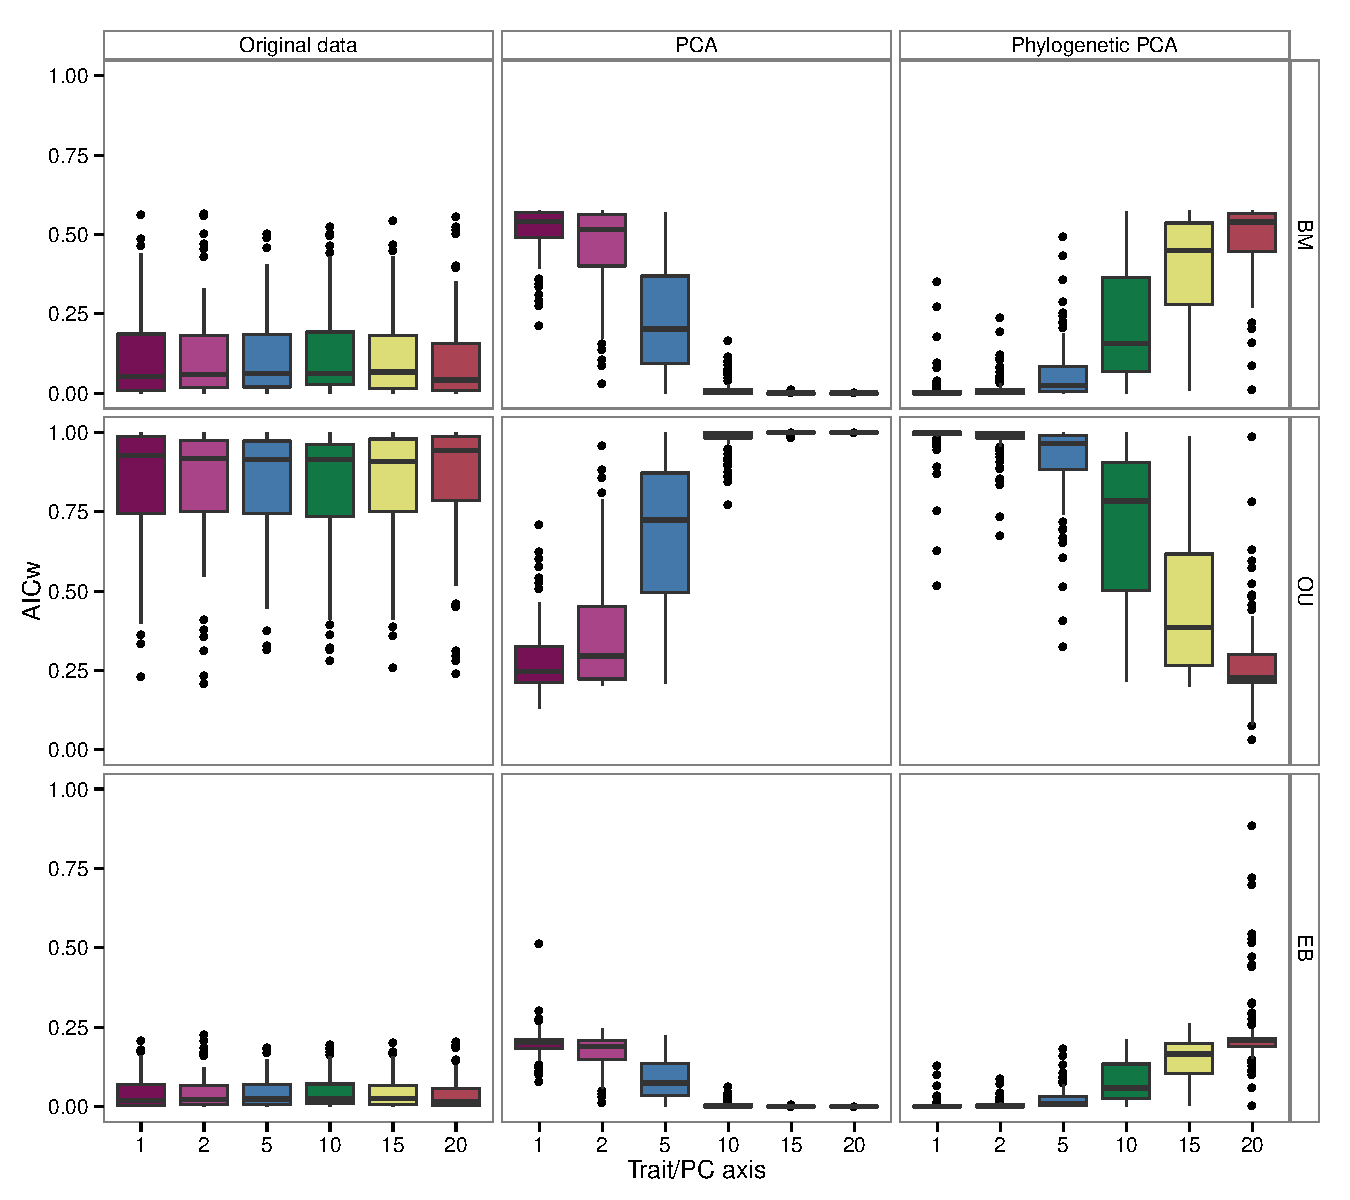
\includegraphics[scale=0.5]{./fig/box-aicw-mvou.pdf}
\caption{}
\label{aicwou}
\end{figure}


\newpage

\bibliographystyle{jecol}
\bibliography{phylopca.bib}
\end{document}
